\documentclass[a4paper,12pt]{article}

\usepackage{cmap}					% поиск в PDF
\usepackage[T2A]{fontenc}			% кодировка
\usepackage[utf8]{inputenc}			% кодировка исходного текста
\usepackage[english,russian]{babel}	% локализация и переносы
\usepackage{enumitem}  				% смена типа символя у enumerate
\usepackage{amsmath,amsfonts,amssymb,amsthm,epsfig,epstopdf,titling,url,array}
\usepackage{icomma} 				% "Умная" запятая: $0,2$ --- число, $0, 2$ --- перечисление
\usepackage{hyperref}				% кликабельные ссылки
\usepackage{soulutf8} 				% Модификаторы начертания
\usepackage{mathtools}
\DeclarePairedDelimiter{\ceil}{\lceil}{\rceil}


\usepackage{multicol, caption}
\usepackage{lipsum}
\newenvironment{Figure}
	{\par\medskip\noindent\minipage{\linewidth}}
	{\endminipage\par\medskip}

\graphicspath { {img} }

\usepackage[ruled,
linesnumbered,
vlined]
{algorithm2e}				% красивые алгоритмы

\sloppy

\SetAlgorithmName{Алгоритм}{algo}{Список алгоритмов}
\SetKwInput{KwData}{Вход}
\SetKwInput{KwResult}{Выход}
\SetNlSty{textbf}{}{.}
\SetAlgoNlRelativeSize{0}
\SetKwIF{If}{ElseIf}{Else}{Если}{то}{иначе если}{иначе}{}
\SetKwFor{ForEach}{Для каждого}{:}{fintq}%
\SetKwFor{While}{Пока}{}{fintq}%

\title{Контрольная работа \linebreak Вариант №4.}
\author{Роман Астраханцев, СКБ-171}

\begin{document}
	\maketitle
	
	\section*{Задача 1}
	Дана сеть Фейстеля, состоящая из 8 итераций, с длиной блока $n=128$ бит.
	Из мастер ключа $K=(K_1, K_2, K_3, K_4)$, где $K_1, \dots, K_4 \in V_{64}$, итерационные ключи (на итерациях $1, 2, 3, \dots, 8$) получаются вырабаютываются как последовательность $K_3, K_2, K_4, K_1, K_3, K_2, K_4, K_1$. Обозначим за $E: V_{128} \times V_{256} \rightarrow V_{128}$ алгоритм зашифрования.
	
	Описать трудоемкость, вероятность успеха, затраты по памяти и объём материала для методов тотального опробования и слайд-атаки.
		
		
	\begin{multicols}{2}
        \begin{Figure}
			\centering
			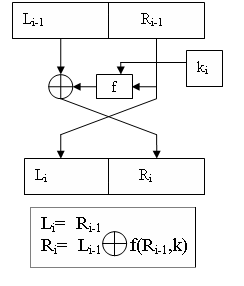
\includegraphics[width=\linewidth]{round.png}
			\captionof{figure}{Раунд сети Фейстеля}
		\end{Figure}

        \begin{Figure}
			\centering
			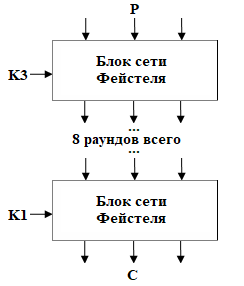
\includegraphics[width=\linewidth]{cpiher.png}
			\captionof{figure}{Шифр из задачи}
		\end{Figure}			
	\end{multicols}

	\subsection*{Метод тотального опробования}
	
	Для начала определим количество материала, необходимое для однозначного опредления ключа. Поскольку одной на паре $(P, C)$ открытого и шифрованного текста, где $P, C \in V_{128}$, можно отбраковать $2^{128}$ ключей, то потребуется $\ceil{\frac{256}{128}} = 2$ различные пары: $(P_1, C_1), (P_2, C_2)$. Будем дальше считать, что они нам даны.
	
	
	\begin{algorithm}[H]
		
		\caption{Метод тотального опробования}
		\label{alg:Total}
		\SetAlgoNoEnd \SetAlgoNoLine 
		
		\KwData{Пары открытого и шифрованного текста $(P_1, C_1), (P_2, C_2)$}
		\KwResult{Ключ шифрования $K$}
		
		\ForEach{$\tilde{k} \in V_{256}$}{ 
			Вычислить $B_1 = E(P_1, \tilde{k})$ \\
			\If{$B_1=C_1$,}{
				Вычислить $B_2 = E(P_2, \tilde{k})$ \\
				\If{$B_2=C_2$,}{
					Закончить алгоритм и вернуть $\tilde{k}$
				}
			}
		}
	\end{algorithm}	
	
	Трудоёмоксть $Q$ этого алгоритма будем измерять в количествах зашифрования, а необходимую для работы алгоритма память $M$ в битах. Тогда имеем
	
	\[ Q = 2^{256} + 2^{128} + 1 \approx 2^{256} \]
	
	\[ M = (128+128)*2 = 512 \]	
	
	Вероятность успеха алгоритма $P = 1$, поскольку алгоритм гарантированно находит ключ шифрования.

	\subsection*{Слайд-атака}
	
	Заметим, что алгоримт зашфирования $E$ представим как $E=G \circ G$, где $G: V_{128} \times V_{256} \rightarrow V_{128}$ -- работа первых 4 раундов сети Фейстеля представленного в задаче шифра. Точно так же, как и в методе тотального опробования, после нахождения слайд-пары необоходимо будет доопробовать найденный ключ. В общем итоге для восстановления ключа нам потребуется $\ceil{\frac{256}{128}} = 2$ различные пары: $(P_1, C_1), (P_2, C_2)$. Будем дальше считать, что они нам даны. Также будем считать, что нам дана возможность по любому открытому тексту получить его зашифрованную версию, иными словами для любого открытого текста $P$ мы можем вычислить $E(P, K)$ даже не зная $K$.
	
		\begin{algorithm}[H]
		
		\caption{Метод скольжения}
		\label{alg:Slide}
		\SetAlgoNoEnd \SetAlgoNoLine 
		
		\KwData{Пары открытого и шифрованного текста $(P_1, C_1), (P_2, C_2)$}
		\KwResult{Ключ шифрования $K$}
		
		Принять $i=1$
		
		\While{ключ не найден или $i > 2^{64}$}{
			
			$i=i+1$
			
			Выберем случайно $P \in V_{128}$ -- открытый текст
			
			Посчитаем $C=E(P, K)$ 
			
			Выберем случайно $P' \in V_{128}$ -- другой открытый текст
			
			Посчитаем $C'=E(P', K)$ 
			
			\If{пары $(P, C)$ и  $(P', C')$ совпали,}{
				Перейти на новую итерацию цикла
			}
			
			Решим уравнение $P'=G(P)$ и результат занесём в $K_{first}$
					
			Решим уравнение $C'=G(C)$ и результат занесём в $K_{last}$
			
			\If{$K_{first}=K_{last}$}{
				Доопробуем ключ $K_{first}$ на парах $(P_1, C_1), (P_2, C_2)$ и в случае успеха вернём ключ $K_{first}$
			}
		}
	\end{algorithm}	

	Алгоритм \ref{alg:Slide} был сформулирован как вероятностный, чтобы продемонстрировать его основные характеристики. Детеременированная версия алгоритма (вероятность успеха которой равна 1) легко получается заменой случайного выбора на перебор всевозможных значений.
	
	Трудоёмоксть $Q$ этого алгоритма будем измерять в количествах зашифрования, а необходимую для работы алгоритма память $M$ в битах. Тогда имеем
	
	\[ Q = 2^{64} \cdot 2q\]
	
	\[ M = (128+128)*2 = 512, \]
	
	где $q$ -- это сложность решения уравнения $P'=G(P)$ относительно ключа $k$. 
	
	Согласно парадоксу дней рождений вероятность успеха алгоритма $P \gg 0.9999$.
	
	
	
\end{document}
